% !Mode:: "TeX:UTF-8"
% !TEX TS-program = XeLaTeX
% !TEX encoding = UTF-8 Unicode

\chapter{\TeX{}中的数学公式编写}\label{chap03}
优美的数学公式是应用\TeX{}进行学术论文撰写的重要原因之一,为达到熟练书写的目的,具备一些数学公式书写语法知识是必要的。关于公式的书写目前也有不少书籍专门论述,例如China\TeX{}主站的Math Mode(\href{http://www.math.ecnu.edu.cn/~latex/docs/Eng_doc/TheLatexCompanionCh8.pdf}{DownLoad Page}),C\TeX{}主站的FAQ问题集(\href{http://www.ctex.org/CTeXFAQ}{DownLoad Page}),以及C\TeX{}套装帮助中也列出了一些对数学公式和特殊符号书写的帮助文件,想在\TeX{}环境下写好公式并非一蹴而就,很多不同领域内所需要的符号,要在论坛或者书籍中反复查找,需要什么样的环境?来自于何种定义?必须加载哪一个宏包?...等等,不一而足。

本节将给出一些基础的公式书写方法,可以对照论文内的源代码,推测出一些论文公式的常见写法。

\section{不同的数学字体}

$\mathbf{A},\mathcal{A},\mathfrak{A},\mathbb{A},\mathscr{A}$

$\mathbf{L},\mathcal{L},\mathfrak{L},\mathbb{L},\mathscr{L}$

\begin{lstlisting}
$\mathbf{A},\mathcal{A},\mathfrak{A},\mathbb{A},\mathscr{A}$
\end{lstlisting}

\section{行内和行间数学模式}
\LaTeX{}有两种特定的模式来排版数学公式,包括行内数学模式和行间数学模式。

行内数学模式将公式排版在一个段落中,使用方式:
\begin{lstlisting}
\(...\)
$...$
\begin{math} ... \end{math}.
\end{lstlisting}

行间数学模式一般用于较长的数学方程或希望单独显示的公式,使用方式为:
\begin{lstlisting}
\[...\]
\begin{displaymath}...\end{displaymath}
\end{lstlisting}

有些符号在这两种模式显示效果有很大不同。一般称行内数学模式显示的格式为文本格式,行间数学模式显示的格式为显示模式。

TexStudio行内数学模式快捷键:\keys{Ctrl}+\keys{Shift}+\keys{M} 行间模式为:\keys{Alt}+\keys{Shift}+\keys{M}

如果希望将方程编号,并在之后使用标签去交叉引用,需要用到equation 环境。注意equation已经是数学环境,所以不需要再里面加入行内或者行间数学标识的美元符号等。

\section{数学模式的群组}
数学模式的群组

大部分数学模式的命令只对其后的一个字符有效,因此,如果希望一个命令对多个字符起作用,必须把它们放在一个群组中,使用花括号:\{\}。例如$e^{i\pi}=1$的代码:
\begin{lstlisting}
e^{i\pi}=1
\end{lstlisting}

\section{数学公式的基本元素}

下面介绍数学排版中比较重要的一些命令。这些命令须包括在数学模式中,即行内的一对美元符号,或行间的反斜杠加中括号。

\subsection{希腊字母}

希腊字母 小写输入$\alpha$, $\beta$, $\gamma$、 大写输入$\Gamma$,$\Theta$, $\Delta$依次为:
\begin{lstlisting}
\alpha, \beta, \gamma
\Gamma,\Theta, \Delta
\end{lstlisting}
\subsection{指数和下标}

指数和下标 可分别通过\^和\_ 两个符号指定,注意:如果指数和下标超过一个字符,需要用到群组。即文本用花括号括起来。惯例是:\hei 先输下标后输指数\song 。

TexStudio中,下标的快捷键为\keys{Ctrl}+\keys{Shift}+\keys{D},指数快捷键为\keys{Ctrl}+\keys{Shift}+\keys{U}

\subsection{平方根}
公式中的平方根$\sqrt{}$、$n$次方根$\sqrt[n]{}$和仅仅只有根号$\surd$的输入方法依次如下:
\begin{lstlisting}
\sqrt{},\sqrt[n]{},\surd
\end{lstlisting}

TexStudio平方根快捷键为\keys{Ctrl}+\keys{Shift}+\keys{Q}。

\subsection{水平线和撇}

水平线$\overline{ABC}$、$\underline{ABC}$和单个字符上方的短横线$\bar{A}$用如下命令实现。
\begin{lstlisting}
\overline{ABC},\underline{ABC},\bar{A}
\end{lstlisting}
用' 可以输入一个撇号。

\subsection{向量}
如下命令依次为向量上的小箭头~$\vec{a}$、以及$A$到$B$的向量~$\overrightarrow{AB}$和$\overleftarrow{AB}$:
\begin{lstlisting}
\vec{a},\overrightarrow{AB},\overleftarrow{AB}
\end{lstlisting}

\subsection{点}
数学符号中的单个点$\cdot$、省略符号点:$\cdots$(中间横向)、$\ldots$(底部横向)、$\vdots$(竖向)和$\ddots$(对角点)分别为:
\begin{lstlisting}
\cdot,\cdots,\ldots,\vdots,\ddots
\end{lstlisting}
一般来说,用在列举时用基线的点,用在相似项相加时用上下居中的点。
\[x_{1},\ldots.x_{n} \quad x_{1}+\cdots + x_{n}\]

\subsection{函数}
函数通常直立字体,\LaTeX{}预制了很多函数命令。例如:$\backslash$log,$\backslash$cos等。

\subsection{取模}
取模有两个命令:$\backslash$bmod 用于二元运算,$\backslash$pmod用于模的方程,例如:$a\bmod b$和$ x\equiv a\pmod{b}$,命令依次为:
\begin{lstlisting}
$a \bmod b$
$ x \equiv a \pmod {b}$
\end{lstlisting}

\subsection{分式}
上下形式的分式基本命令为$\backslash$frac。amsmath提供了另外两种命令$\backslash$dfrac和$\backslash$tfrac , 前者无论行间环境还是行内环境都打印显示模式,后者则无论行间还是行内都打印文本模式。 一般对较小的分式可以直接输入/。

例如行内模式下$\frac{1}{k}$、$\dfrac{1}{k}$和$\tfrac{1}{k}$为:
\begin{lstlisting}
$\dfrac{1}{k} \; \frac{1}{k} \; \tfrac{1}{k}$
\end{lstlisting}
显示模式下,\[\dfrac{1}{k} \; \frac{1}{k} \; \tfrac{1}{k}\]表示为:
\begin{lstlisting}
\[ \dfrac{1}{k} \; \frac{1}{k} \; \tfrac{1}{k}\]
\end{lstlisting}
TexStudio的$\backslash$frac快捷键为\keys{Alt}+\keys{Shift}+\keys{F};dfrac 快捷键:\keys{Ctrl}+\keys{Shift}+\keys{F};跳到下一个可编辑区域,例如从分子编辑区域跳到分母编辑区,快捷键为:\keys{Ctrl}+\keys{→}。

\subsection{积分}
积分、求和与乘积的符号分别用前置反斜杠加$\backslash$int, $\backslash$sum, $\backslash$prod表示,其中\^和\_表示上限和下限,例如:
\begin{equation}\label{eq:intsumprod}
\left\{
\begin{aligned}
&f(x)=\sum_{n=0}^{\infty}a_nx^n\\
&\int_{0}^{a}x+n\mathrm{d}x\\
&f(x)=\prod_{i=1}^{n}x^i
\end{aligned}
\right.
\end{equation}
代码为:
\begin{lstlisting}
\begin{equation}
\left\{
\begin{aligned}
&f(x)=\sum_{n=0}^{\infty}a_nx^n\\
&\int_{0}^{a}x+n\mathrm{d}x\\
&f(x)=\prod_{i=1}^{n}x^i
\end{aligned}
\right.
\end{equation}
\end{lstlisting}
重积分$\iint$, $\iiint$,$\idotsint$代码则依次为:
\begin{lstlisting}
$\iint$, $\iiint$,$\idotsint$
\end{lstlisting}
\subsection{定界符}
定界符的小括号和中括号可直接打出,大括号需要前置反斜杠转义,即:$\backslash\{\backslash\}$

需要调整定界符的大小时,在左定界符前加$\backslash$left , 并在右定界符前加$\backslash$right 。\LaTeX 会自动调整定界符大小,如:\[(\prod_{i=1}^{n})x_{i} ) \quad \left(\prod_{i=1}^{n} x_{i}\right)\]代码为:
\begin{lstlisting}
\[(\prod_{i=1}^{n})x_{i} ) \quad \left(\prod_{i=1}^{n} x_{i}\right)\]
\end{lstlisting}
有时候自动调整效果不满意,可以使用$\backslash$big, $\backslash$Big, $\backslash$bigg, $\backslash$Bigg来调整。

TexStudio中,$\backslash$left快捷键为:\keys{Ctrl}+\keys{Shift}+\keys{L} , $\backslash$right快捷键为:\keys{Ctrl}+\keys{Shift}+\keys{R}。

\subsection{数学空格}
有时候\TeX{}选择的空格不令人满意,可插入一些特殊空格控制命令调整。空格由小到大依次为$\backslash$,、$\backslash$:、$\backslash$;、$\backslash$quad和$\backslash$qquad 。

在重积分的空格选取中,amsmath提供了$\backslash$iint、$\backslash$iiint、$\backslash$iiiint和$\backslash$idotint 来生成重积分号。

\subsection{矩阵}
amsmath宏包提供了一系列用于排版的矩阵环境,都依托于\LaTeX{}中的array 环境。
\begin{table}[htbp]
	\bicaption[tab:Matrix]{表}{数学公式中的矩阵表述}{Tab.}{Describtion of matrix in math}
	\centering
	\vspace{0.2cm}
	\zhongwu
	\begin{tabular}{cc}
		\toprule
		环境  & 矩阵 \\
		\midrule
		pmatrix   &     ()   \\
		bmatrix   &     []   \\
		Bmatrix	  &   \{\}   \\
		vmatrix   &          \\
		Vmatrix   &          \\ 
		\bottomrule
	\end{tabular}
\end{table}

同样也提供了用于生成行内数学模式中的小矩阵环境smallmatrix,此外,矩阵环境中的下一列和换行命令与表格中一致,例如:
\[ \det(A)=\begin{vmatrix}
a_{11} & a_{12} & \cdots  & a_{1n}\\
a_{21} & a_{22} & \cdots  & a_{2n}\\
\cdots & \cdots & \cdots  & \cdots\\
a_{n1} & a_{n2} & \cdots  & a_{nn}\\
\end{vmatrix} \]的\TeX{}代码为:
\begin{lstlisting}
\[ \det(A)=\begin{vmatrix}
a_{11} & a_{12} & \cdots  & a_{1n}\\
a_{21} & a_{22} & \cdots  & a_{2n}\\
\cdots & \cdots & \cdots  & \cdots\\
a_{n1} & a_{n2} & \cdots  & a_{nn}\\
\end{vmatrix} \]
\end{lstlisting}

\subsection{分段函数}
amsmath宏包提供了cases 环境用于方便排版分段函数,例如公式:
\[ \delta(x)=\begin{cases}
1   &x=0,\\
0  & x\neq0.
\end{cases} \]\TeX{}代码为:
\begin{lstlisting}
\[ \delta(x)=\begin{cases}
1   &x=0,\\
0  & x\neq0.
\end{cases} \]
\end{lstlisting}
当然它也可以由aligned环境人为定义:
\begin{lstlisting}
\begin{equation*}\label{alignedfun}
\delta(x)=\left\{
\begin{aligned}
1\qquad   &x=0,\\
0\qquad   & x\neq0.	
\end{aligned}
\right.
\end{equation*}
\end{lstlisting}
这段代码中使用了equation*环境,它也是无编号公式,和$\backslash$[...$\backslash$]功效相同。

\subsection{长公式}
amsmath宏包提供了很多用于长公式排版的命令,一般基于\LaTeX 的equation和eqnarry 环境。但amsmath文档建议不再使用长公式环境。

公式环境中,命令$\backslash$tag\{num\}可生成公式编号。命令$\backslash$notag 取消公式的编号。

\subsection{公式子编号}
环境subequations 可以生成类似(4.9 a),(4.9 b)之类的编号。
\begin{subequations}
	\begin{align}
	(1-\mu_{x}\delta_{x}^2)U^{n+1/2}_j&=(1+\frac{1}{2}\mu_y\delta_y^2 )U^n_j \\
	(1-\mu_y\delta_y^2)U^{n+1}_j&=(1+\frac{1}{2}\mu_x\delta_x^2)U^{n+1/2}_j
	\end{align}
\end{subequations}
上述公式可通过下列代码实现:
\begin{lstlisting}
\begin{subequations}
\begin{align}
(1-\mu_{x}\delta_{x}^2)U^{n+1/2}_j&=(1+\frac{1}{2}\mu_y\delta_y^2 )U^n_j \\
(1-\mu_y\delta_y^2)U^{n+1}_j&=(1+\frac{1}{2}\mu_x\delta_x^2)U^{n+1/2}_j
\end{align}
\end{subequations}
\end{lstlisting}
如果中间再加上部分文字,比如:
\begin{subequations}
	\begin{align}
	x&=1+3\\
	\intertext{wo}\notag\\
	y&=x+2\\
	z&=x+y
	\end{align}
\end{subequations}
实现的\TeX{}代码:
\begin{lstlisting}
\begin{subequations}
\begin{align}
x&=1+3\\
\intertext{wo}\notag\\
y&=x+2\\
z&=x+y
\end{align}
\end{subequations}
\end{lstlisting}








%\subsection{行内公式和无编号公式}
%行内公式,相当于公式编辑器mathtype中的“inline”型公式,在\TeX{}语法中,公式主体包裹在一对美元符号内,例如$\sqrt[3]{{x_1}^2+{y_1}^2}$,由如下方式定义:
%\begin{lstlisting}
%	$\sqrt[3]{{x_1}^2+{y_1}^2}$
%\end{lstlisting}
%无编号公式(display mode)和行内公式的区别在于它要独占一行,但没有相应编号,它的公式主体要包括在一对反斜杠中括号之内。类似于公式编辑器mathtype中的display型公式,例如下面的无编号公式:\[\Delta f=\dfrac{\partial^2f}{\partial x^2}+\dfrac{\partial^2f}{\partial x^2}\]由如下方式定义:
%\begin{lstlisting}
%\[\Delta f=\dfrac{\partial^2f}{\partial x^2}+
%	\dfrac{\partial^2f}{\partial y^2}\]
%\end{lstlisting}
%\subsection{带编号公式}
%编号公式是一个equation环境,例如柱坐标系下的拉普拉斯算子如式\ref{eq:laplace}所示:
%\begin{equation}\label{eq:laplace}
%	\Delta f=\dfrac1\rho\dfrac{\partial}{\partial \rho}\left(\rho\dfrac{\partial f}{\partial\rho}\right)+
%	\dfrac{1}{\rho^2}\dfrac{\partial^2f}{\partial \theta^2}+
%	\dfrac{\partial^2f}{\partial z^2}
%\end{equation}
%公式\ref{eq:laplace}的主体被包括在如下环境中:
%\begin{lstlisting}
%\begin{equation}\label{eq:laplace}
%\Delta f=\dfrac1\rho\dfrac{\partial}{\partial\rho}
%\left(\rho\dfrac{\partial f}{\partial\rho}\right)+
%\dfrac{1}{\rho^2}\dfrac{\partial^2f}{\partial \theta^2}+
%\dfrac{\partial^2f}{\partial z^2}
%\end{equation}
%\end{lstlisting}

%\subsection{傅立叶变换}
%
%在现代数学中有一个很容易被外行误解的词汇:信号 (signal)。当数学家们说起
%「一个信号」的时候,他们脑海中想到的并不是交通指示灯所发出的闪烁光芒或者
%手机屏幕顶部的天线图案,而是一段可以具体数字化的信息,可以是声音,可以是
%图像,也可是遥感测量数据。简单地说,它是一个函数,定义在通常的一维或者多
%维空间之上。譬如一段声音就是一个定义在一维空间上的函数,自变量是时间,因
%变量是声音的强度,一幅图像是定义在二维空间上的函数,自变量是横轴和纵轴坐
%标,因变量是图像像素的色彩和明暗,如此等等\footnote{木遥:不确定性原理的
%  前世今生 · 数学篇(一)}。
%
%在数学上,关于一个信号最基本的问题在于如何将它表示和描述出来。按照上面所
%说的办法,把一个信号理解成一个定义在时间或空间上的函数是一种自然而然的表
%示方式,但是它对理解这一信号的内容来说常常不够。例如一段声音,如果单纯按
%照定义在时间上的函数来表示,它画出来是这个样子的:
%
%\begin{figure}[htbp]
%  \centering
%  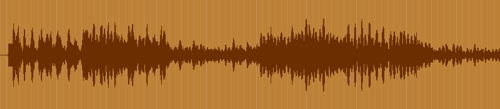
\includegraphics[width=0.8\textwidth{},keepaspectratio]{VisualAudio.png}
%  \bicaption[fig:boxingtu]{波形图}{波形图}{Fig.}{Wave}
%\end{figure}
%
%图~\ref{fig:boxingtu}通常被称为波形图。毫无疑问,它包含了关于这段声音的全
%部信息。但是同样毫无疑问的是,这些信息几乎没法从上面这个「函数」中直接看
%出来,事实上,它只不过是巴赫的小提琴无伴奏 Partita No.3 的序曲开头几个小
%节。图~\ref{fig:bahe} 是巴赫的手稿,从某种意义上说来,它也构成了对上面那
%段声音的一个「描述」:
%
%\begin{figure}[htbp]
%  \centering
%  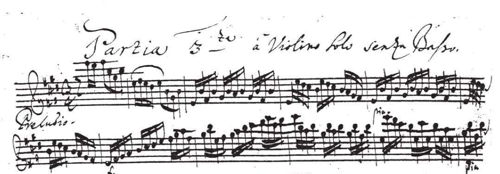
\includegraphics[width=0.8\textwidth{},keepaspectratio]{Partita3.png}
%  \bicaption[fig:bahe]{巴赫手稿}{巴赫手稿}{Fig.}{Partita No.3}
%\end{figure}
%
%这两种描述之间的关系是怎样的呢?第一种描述刻划的是具体的信号数值,第二种
%描述刻划的是声音的高低(即声音震动的频率)。人们直到十九世纪才渐渐意识到,
%在这两种描述之间,事实上存在着一种对偶的关系,而这一点并不显然。
%
%1807 年,法国数学家傅立叶 (J. Fourier) 提出了一个崭新的观念:任何一个函数
%都可以表达为一系列不同频率的简谐振动(即简单的三角函数)的叠加。
%
%用今天的语言来描述,傅立叶的发现实际上是在说:任何一个信号都可以用两种方
%式来表达,一种就是通常意义上的表达,自变量是时间或者空间的坐标,因变量是
%信号在该处的强度,另一种则是把一个信号「展开」成不同频率的简单三角函数
%(简谐振动)的叠加,于是这就相当于把它看作是定义在所有频率所组成的空间
%(称为频域空间)上的另一个函数,自变量是不同的频率,因变量是该频率所对应
%的简谐振动的幅度。
%
%
%这两个函数一个定义在时域(或空域)上,一个定义在频域上,看起来的样子通常
%截然不同,但是它们是在以完全不同的方式殊途同归地描述着同一个信号。它们就
%象是两种不同的语言,乍一听完全不相干,但是其实可以精确地互相翻译。在数学
%上,这种翻译的过程被称为「傅立叶变换」。
%
%傅立叶变换是一个数学上极为精美的对象:
%\begin{enumerate}
%\item 它是完全可逆的,任何能量有限的时域或空域信号都存在唯一的频域表达,
%  反之亦然 。
%\item 它完全不损伤信号的内在结构:任何两个信号之间有多少相关程度(即内
%  积),它们的频域表达之间也一定有同样多的相关程度。
%\item 它不改变信号之间的关联性:一组信号收敛到一个特定的极限,它们的频域
%  表达也一定收敛到那个极限函数的频域表达。
%\end{enumerate}
%
%在傅立叶变换的所有这些数学性质中,最不寻常的是这样一种特性:一个在时域或
%空域上看起来很复杂的信号(譬如一段声音或者一幅图像)通常在频域上的表达会
%很简单。这里「简单」的意思是说作为频域上的函数,它只集中在很小一块区域内,
%而很大一部分数值都接近于零。
%
%一个在空域中看起来占满全空间的信号,从频域中看起来很可能只不过占用了极小
%一块区域,而大部分频率是被浪费了的。这就导出了一个极为有用的结论:一个看
%起来信息量很大的信号,其实可以只用少得多的数据来加以描述。只要对它先做傅
%立叶变换,然后只记录那些不接近零的频域信息就可以了,这样数据量就可以大大
%减少。
%
%基本上,这正是今天大多数数据压缩方法的基础思想。在互联网时代,大量的多媒
%体信息需要在尽量节省带宽和时间的前提下被传输,所以数据压缩从来都是最核心
%的问题之一。而今天几乎所有流行的数据压缩格式,无论是声音的 mp3 格式还是图
%像的 jpg 格式,都是利用傅立叶变换才得以发明的。从这个意义上说来,几乎全部
%现代信息社会都建立在傅立叶的理论的基础之上。